%----------------------------------------------------------------------------------------
%    PACKAGES AND THEMES
%----------------------------------------------------------------------------------------
\documentclass[aspectratio=169,xcolor=dvipsnames]{beamer}
\makeatletter
\def\input@path{{theme/}}
\makeatother
\usetheme{CleanEasy}
\usepackage[utf8]{inputenc}
\usepackage{lmodern}
\usepackage[T1]{fontenc}
% \usepackage[brazil]{babel}
\usepackage{fix-cm}
\usepackage{amsmath}
\usepackage{mathtools}
\usepackage{listings}
\usepackage{xcolor}
\usepackage{hyperref}
\usepackage{graphicx} % Allows including images
\usepackage{booktabs} % Allows the use of \toprule, \midrule and \bottomrule in tables
\usepackage{tikz}
\usetikzlibrary{positioning, shapes, arrows, calc, decorations.pathreplacing, arrows.meta, backgrounds, patterns, overlay-beamer-styles}
\usepackage{etoolbox}
\usepackage{animate}
\usepackage{fontawesome5}



\usepackage{pifont}
\usepackage{xcolor}

\newcommand{\cmark}{\textcolor{green}{\ding{51}}}
\newcommand{\xmark}{\textcolor{red}{\ding{55}}}

%----------------------------------------------------------------------------------------
%    LAYOUT CONFIGURATION
%----------------------------------------------------------------------------------------
\input{configs/configs}
%----------------------------------------------------------------------------------------
%    TITLE PAGE
%----------------------------------------------------------------------------------------


\title[Learning-Guided Optimization]{Learning-Guided Mathematical Optimization:\\Methods and Applications}

\author[Ankur Nath]{Ankur Nath}

\institute[TAMU]{%
  Department of Computer Science \& Engineering\\
  Texas A\&M University
}

\date{May 2026}

\titlegraphic{
  \begin{tikzpicture}[remember picture, overlay]
    \node[anchor=south west, xshift=0.5cm, yshift=0.2cm] at (current page.south west) {
      
\includegraphics[height=1.1cm]{logos/tamu_logo.png}
    };
  \end{tikzpicture}
}

%----------------------------------------------------------------------------------------


\begin{document}

\begin{frame}[plain]
  \titlepage
\end{frame}

\begin{frame}[plain]{Why Reduce the Search Space of Combinatorial Optimization on Graphs?}
    \centering
    \textbf{\large }
    \vspace{0.5cm}
    
    \begin{columns}[T,onlytextwidth]
        % Left Column
        \column{0.48\textwidth}
        \textbf{\textcolor{blue}{Motivation}}
        \begin{itemize}
            \item[\faTasks] Common tasks: Max Cover, Influence Maximization, TSP
            \item[\faFilter] Many elements irrelevant to solution
            \item[\faBolt] Smaller search space $\rightarrow$ faster computation
        \end{itemize}
        
        % Right Column
        \column{0.48\textwidth}
        \textbf{\textcolor{red}{Challenges}}
        \begin{itemize}
            \item[\faExclamationTriangle] NP-hard problems
            \item[\faProjectDiagram] Graphs with billions of nodes
        \end{itemize}
    \end{columns}
\end{frame}

\begin{frame}[plain]{Motivating Example}
    \small
    \begin{columns}[T,onlytextwidth]
        % Left column: Text
        \column{0.55\textwidth}
        Consider the problem of selecting \textbf{influential individuals} in a social network 
        to receive free product samples, aiming to trigger a cascade of product adoptions 
        through \textbf{word of mouth}.
        
        \vspace{0.3cm}
        Many individuals are poor candidates for selection, such as those with 
        \textit{limited social connections}.
        
        \vspace{0.3cm}
        Instead of considering the \textbf{entire population}, we can focus on a 
        \textbf{smaller subset of highly influential individuals} who are more likely 
        to reach a broad and diverse audience.
        $$\max_{|S| \le k} f(S)$$
        
        % Right column: Figure
        \column{0.45\textwidth}
        \centering
        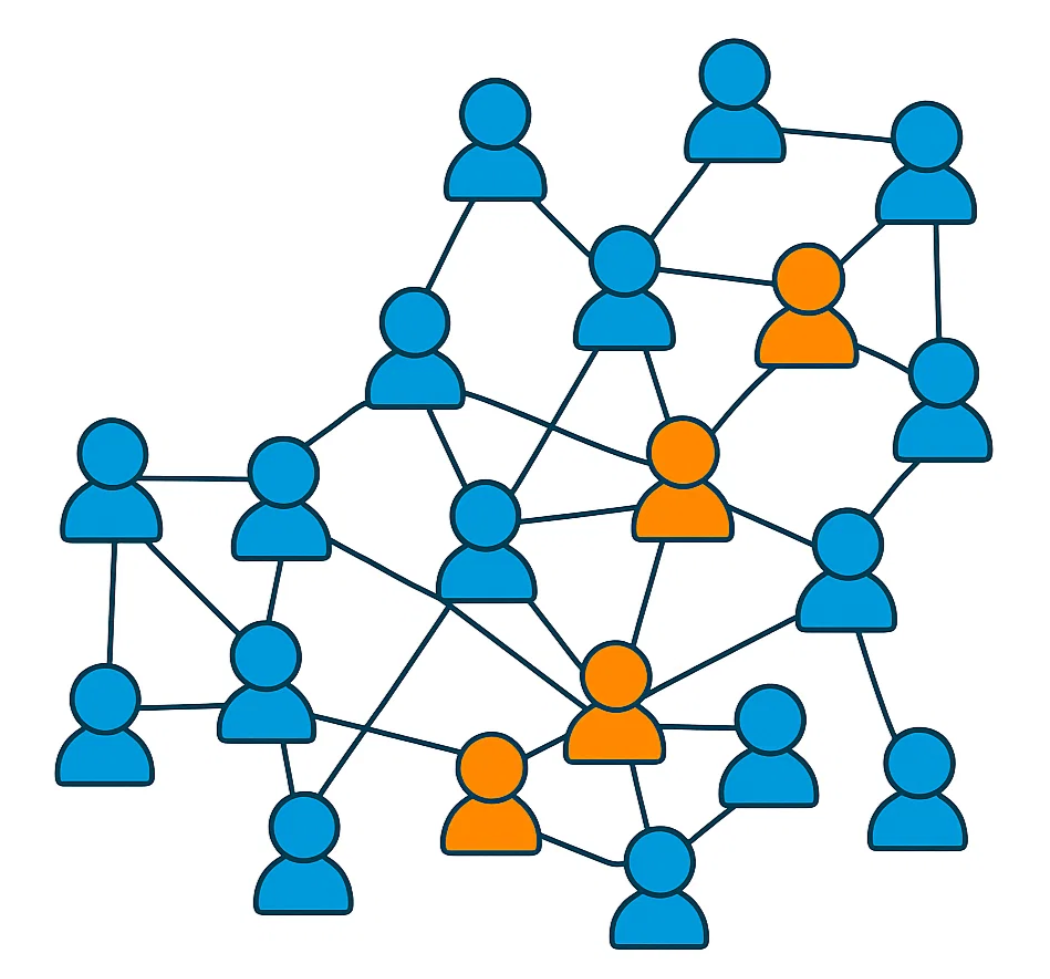
\includegraphics[width=\linewidth]{logos/influence_maximization.PNG} % Replace with your figure path
    \end{columns}
\end{frame}

\begin{frame}[plain]{ \faCut Pruning}

  We are given a combinatorial optimization problem consisting of a ground set \(\mathcal{U}\) and an exact method \(\mathcal{OPT}\) for the problem. An optimal solution is defined as a subset of the ground set \(X^\star = \mathcal{OPT} (\mathcal{U}) \) that maximizes the objective function \(f(\cdot)\) while satisfying the size constraint \(|X| \leq B\), i.e


\[X^\star  = \text{arg max}_{X \subset  \mathcal{U},|X|\leq B} f(X)\]

The problem we aim to address is finding a significantly smaller ground set \(\mathcal{U}'\), such that \(|\mathcal{U}'| \ll |\mathcal{U}|\), while ensuring that the objective value remains unchanged, i.e.,  
\[
\frac{f(\mathcal{OPT}(\mathcal{U}'))}{f(\mathcal{OPT}(\mathcal{U}))} \ge 1 - \epsilon  \]

    
\end{frame}



\begin{frame}[plain]{\faCut Pruning}

\faLightbulbO\ \textbf{ Key Idea:}  
\vspace{0.2cm}

\begin{itemize}
    \item[\faBolt] Quickly discard elements unlikely to be part of an optimal solution
    \item[\faLock] \textbf{Preserve search quality} while improving efficiency
\end{itemize}

    
\end{frame}

\begin{frame}[plain]{Pruning CO Problems: Approaches \& Limitations}

\begin{columns}[T,onlytextwidth]

% Left Column: Categories
\column{0.5\textwidth}
\textbf{Pruning Approaches}
\vspace{0.2cm}
\begin{itemize}
    \item \textbf{Supervised Learning}
    \begin{itemize}
        \item Handcrafted features.
        \item Binary classifiers to prune nodes/edges.
        \item [\textcolor{red}{\xmark}] Needs domain knowledge.
    \end{itemize}

    \vspace{0.2cm}
    \item \textbf{Supervised + RL}
    \begin{itemize}
        \item Learns pruning + solution policies.
        \item Combines GNNs with search.
        \item [\textcolor{red}{\xmark}] Problem-specific tuning.
    \end{itemize}
\end{itemize}

% Right Column: Examples & Drawbacks
\column{0.5\textwidth}
\textbf{Examples}
\vspace{0.2cm}
\begin{itemize}
    \item \textbf{LeNSE} \cite{ireland2022lense}: GNN + local search.
    \item \textbf{GCOMB} \cite{manchanda2020gcomb}: Degree heuristic + Q-learning.
    \item \textbf{COMBHelper} \cite{tian2024combhelper}: GNN + Fourier features.
    

    \vspace{0.3cm}
    \textbf{Common Issues}
    \begin{itemize}
        \item [\textcolor{red}{\xmark}] Not generalizable.
        \item [\textcolor{red}{\xmark}] Costly feature design.
        \item [\textcolor{red}{\xmark}] Needs expert tuning.
    \end{itemize}
\end{itemize}

\end{columns}

\end{frame}

\begin{frame}[plain]{Our Approach: Generalizable Pruning Without Handcrafting}

\begin{columns}[T,onlytextwidth]
    \column{0.48\textwidth}
    \textbf{GCOMB, COMBHelper, LeNSE}
    \vspace{0.2cm}
    \begin{itemize}
        \item [\textcolor{red}{\xmark}] Handcrafted heuristics/features.
        \item [\textcolor{red}{\xmark}] Problem-specific tuning.
        \item [\textcolor{red}{\xmark}] High computational overhead.
        \item [\textcolor{red}{\xmark}] Limited scalability \& adaptability.
    \end{itemize}

    \column{0.52\textwidth}
    \textbf{Our Approach}
    \vspace{0.2cm}
    \begin{itemize}
        \item [\textcolor{green}{\cmark}] Prunes $>$95\% of ground set.
        \item [\textcolor{green}{\cmark}] Best mean combined metric across tasks.
        \item [\textcolor{green}{\cmark}] No handcrafted features.
        \item [\textcolor{green}{\cmark}] Problem-agnostic and lightweight.
        \item [\textcolor{green}{\cmark}] Robust across distributions and CO problems.
    \end{itemize}

\end{columns}

\end{frame}







\begin{frame}[plain]{Hierarchical DeepPruner}

\begin{figure}
    \centering
    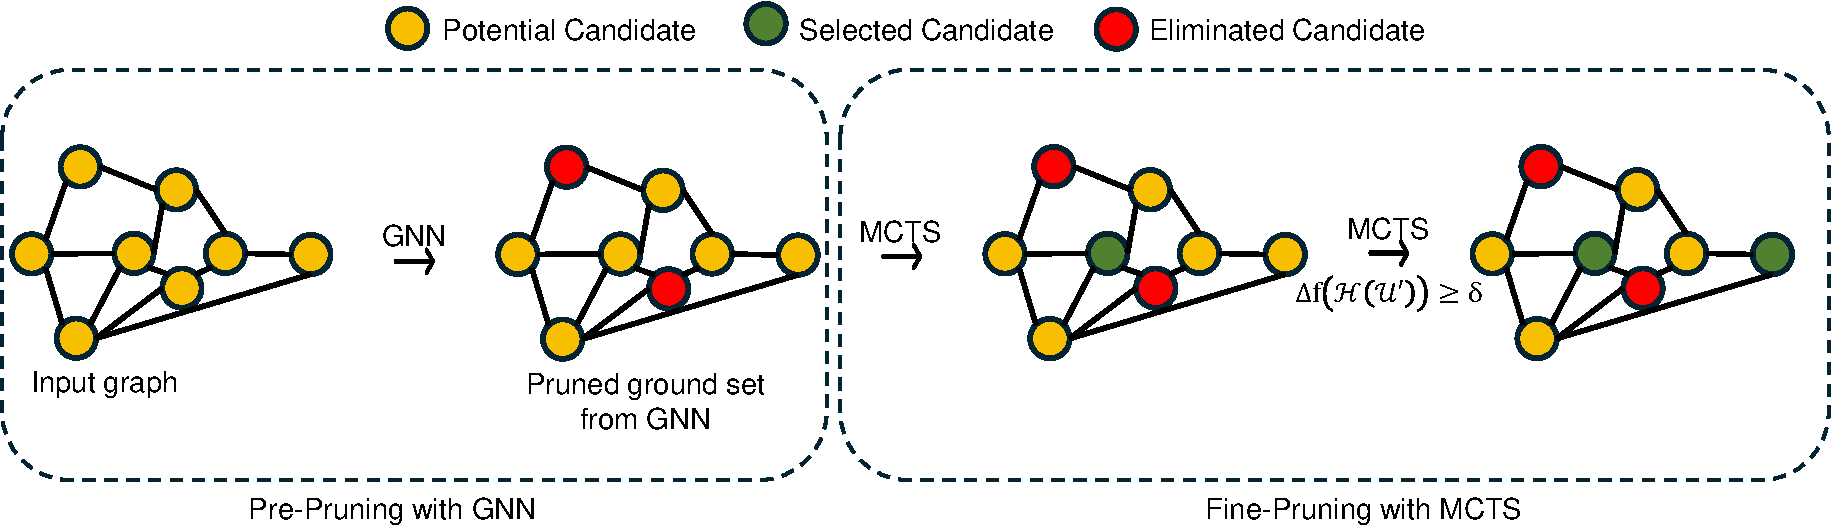
\includegraphics[width=\linewidth]{logos/H_deeppruner_cropped.pdf}
\end{figure}

    
\end{frame}

\begin{frame}[plain]{First Stage: GNN-Based Pre-Pruning}
\begin{itemize} 
    \item [\faBullseye] \textbf{Goal:} Eliminate nodes unlikely to belong to the solution set before running NMCTS.
    \item [\faLightbulb] \textbf{Key Insight:} Nodes in the optimal set often share \textbf{local structural patterns}.
    \item [\faBolt] \textbf{Innovation:} 
    \begin{itemize}
        \item Replace handcrafted heuristics (e.g., TOP-K) with a trainable GNN.
        \item Use random node initialization: \( h_{v_i} \sim U(0,1) \), avoiding problem-specific features.
    \end{itemize}
    \item [\faDatabase] \textbf{Training Setup:}
    \begin{itemize}
        \item ER graphs ($n=2000$, $p=0.1$), budget = $100$.
        \item Ground-truth labels from heuristic solver.
    \end{itemize}
    \item [\faBalanceScale] \textbf{Loss Function:} Weighted cross-entropy to avoid class imbalance (non-solution nodes).
    \item [\faCogs] \textbf{Model:} 2-layer GCN. Other GNNs like GraphSAGE underperform due to limited neighborhood sampling.
\end{itemize}
\end{frame}


\begin{frame}[plain]{GNN Pre-Pruning: Inference \& Efficiency}
\begin{itemize}
    \item [\faForward] \textbf{Inference:} One forward pass over the graph to predict node inclusion probabilities.
    \item [\faCut] \textbf{Pruning Rule:} Discard nodes predicted to belong to the negative class (i.e., not part of the solution).

    \item [\faRocket] \textbf{Efficiency:}
    \begin{itemize}
        \item Significantly reduces ground set size before NMCTS.
        \item Accelerates search without harming objective value.
    \end{itemize}
    \item [\faExclamationTriangle] \textbf{Trade-off:} Slight increase in computation during training due to full-neighborhood GCN.
    \item [\faCheckCircle] \textbf{Justification:} Training is performed only once; inference is lightweight and fast.
\end{itemize}
\end{frame}

\begin{frame}[plain]{Second Stage: Fine-Pruning with MCTS}
\begin{figure}
    \centering
    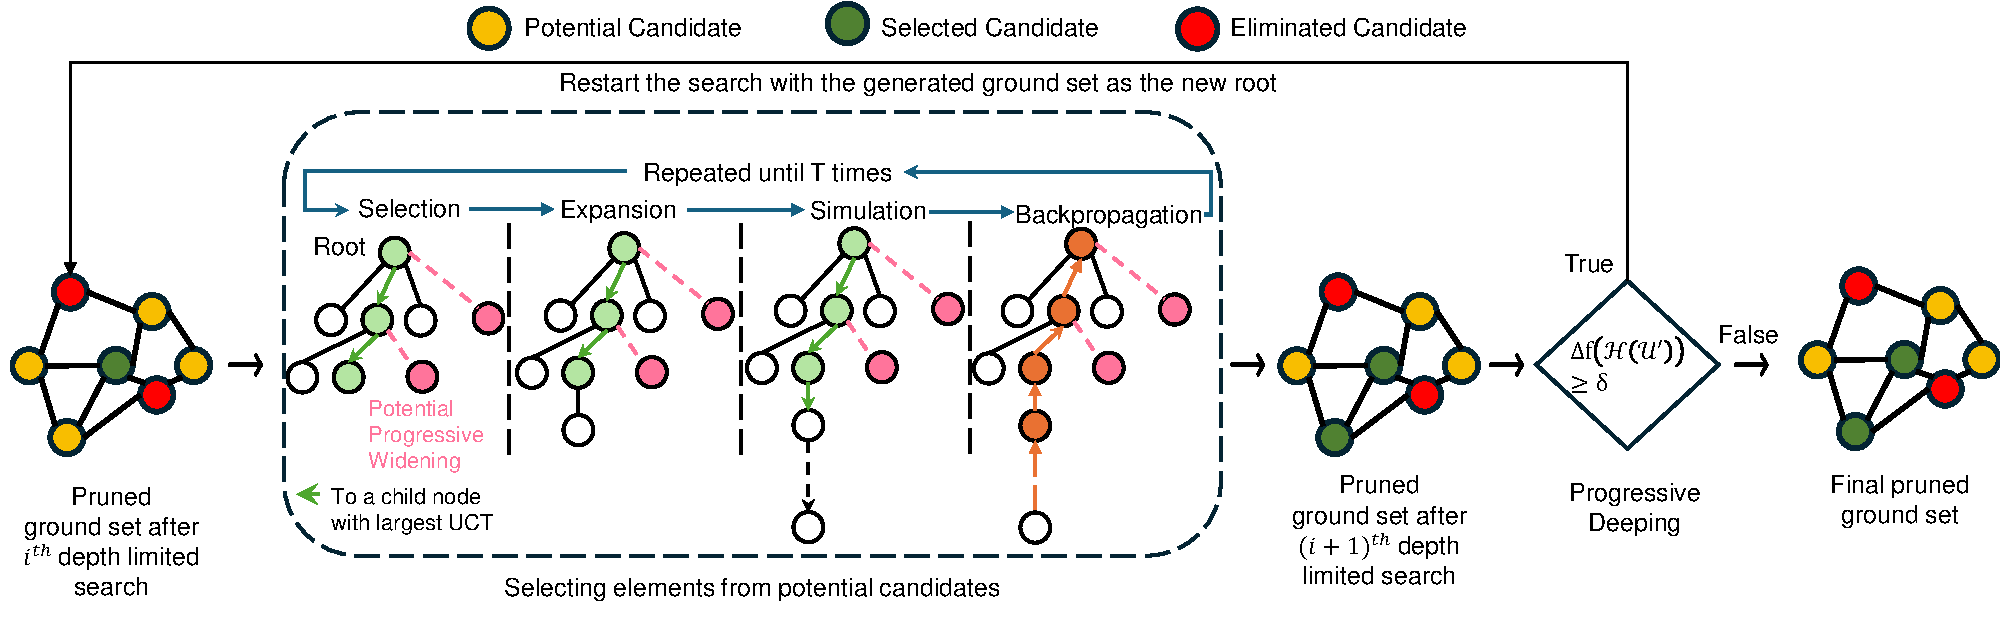
\includegraphics[width=\linewidth]{logos/MCTS_cropped.pdf}
\end{figure}

    
\end{frame}


\begin{frame}[plain]{Second Stage: NMCTS for Refined Pruning}
\begin{itemize}
    \item [\faBullseye] \textbf{Goal:} Refine the pruned set $\mathcal{U}_{\text{GNN}}$ from GNN by considering relative element importance.
    \item [\faExclamation] \textbf{Limitation of GNN:}
    \begin{itemize}
        \item GNN predicts inclusion independently, ignoring interactions.
        \item E.g., if both $v_1$ and $v_2$ are in $\mathcal{U}_{\text{GNN}}$ but contribute equivalently, one can be safely removed.
    \end{itemize}
    \item [\faSitemap] \textbf{Approach:}
    \begin{itemize}
        \item Use NMCTS (Neural Monte Carlo Tree Search) to build a high-quality subset iteratively.
        \item GNN guides initial policy; solution is constructed by adding one element at a time.
        \item Trained on the same ER graphs as the GNN.
    \end{itemize}
    \item [\faRandom] \textbf{Output:} Variable-size pruned set informed by GNN predictions \& adaptive search.
\end{itemize}
\end{frame}

\begin{frame}[plain]{NMCTS with Progressive Refinement}
\begin{itemize}
    \item [\faBullseye] \textbf{Objective:} Refine the GNN-pruned set by sequentially constructing high-quality subsets.
    \item [\faSitemap] \textbf{Approach:} Guide \textbf{Neural MCTS (NMCTS)} with GNN priors to explore promising selections.
    \item [\faSearch] \textbf{Progressive Widening:} 
    \begin{itemize}
        \item Gradually increase explored actions as parent node visits grow.
        \item Add child node if $\lfloor \text{Visits}(N_p)^\alpha \rfloor \geq |\text{CHILDREN}(N_p)|$.
        \item Set $\alpha = 0.1$ in all experiments.
    \end{itemize}
    \item [\faLevelUpAlt] \textbf{Progressive Deepening:} 
    \begin{itemize}
        \item Start from an empty set, search up to depth $50$.
        \item Restart from root if objective improves $\geq 1\%$.
        \item Halt if no significant gain to avoid unnecessary expansion.
    \end{itemize}
    \item [\faChartLine] \textbf{Outcome:} Yields a compact, high-quality subset with minimal loss in objective value.
\end{itemize}
\end{frame}















\begin{frame}[plain]{Empirical Evaluation}
\begin{figure}
    \centering
    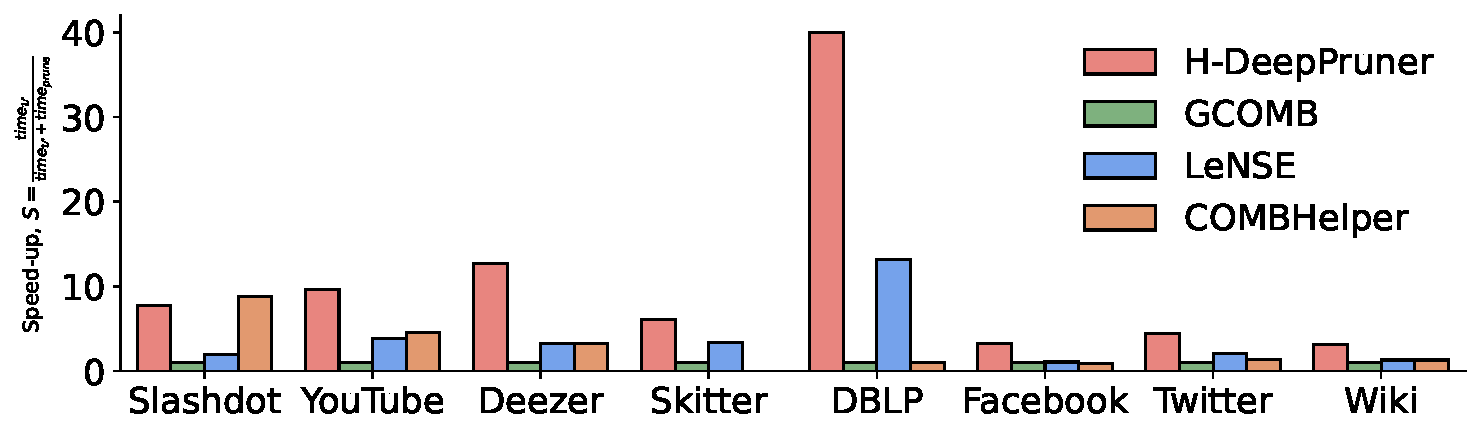
\includegraphics[width=\linewidth]{logos/speed_up.pdf}
\end{figure}

    
\end{frame}


\begin{frame}[plain]{Empirical Evaluation}

\begin{figure}
    \centering
    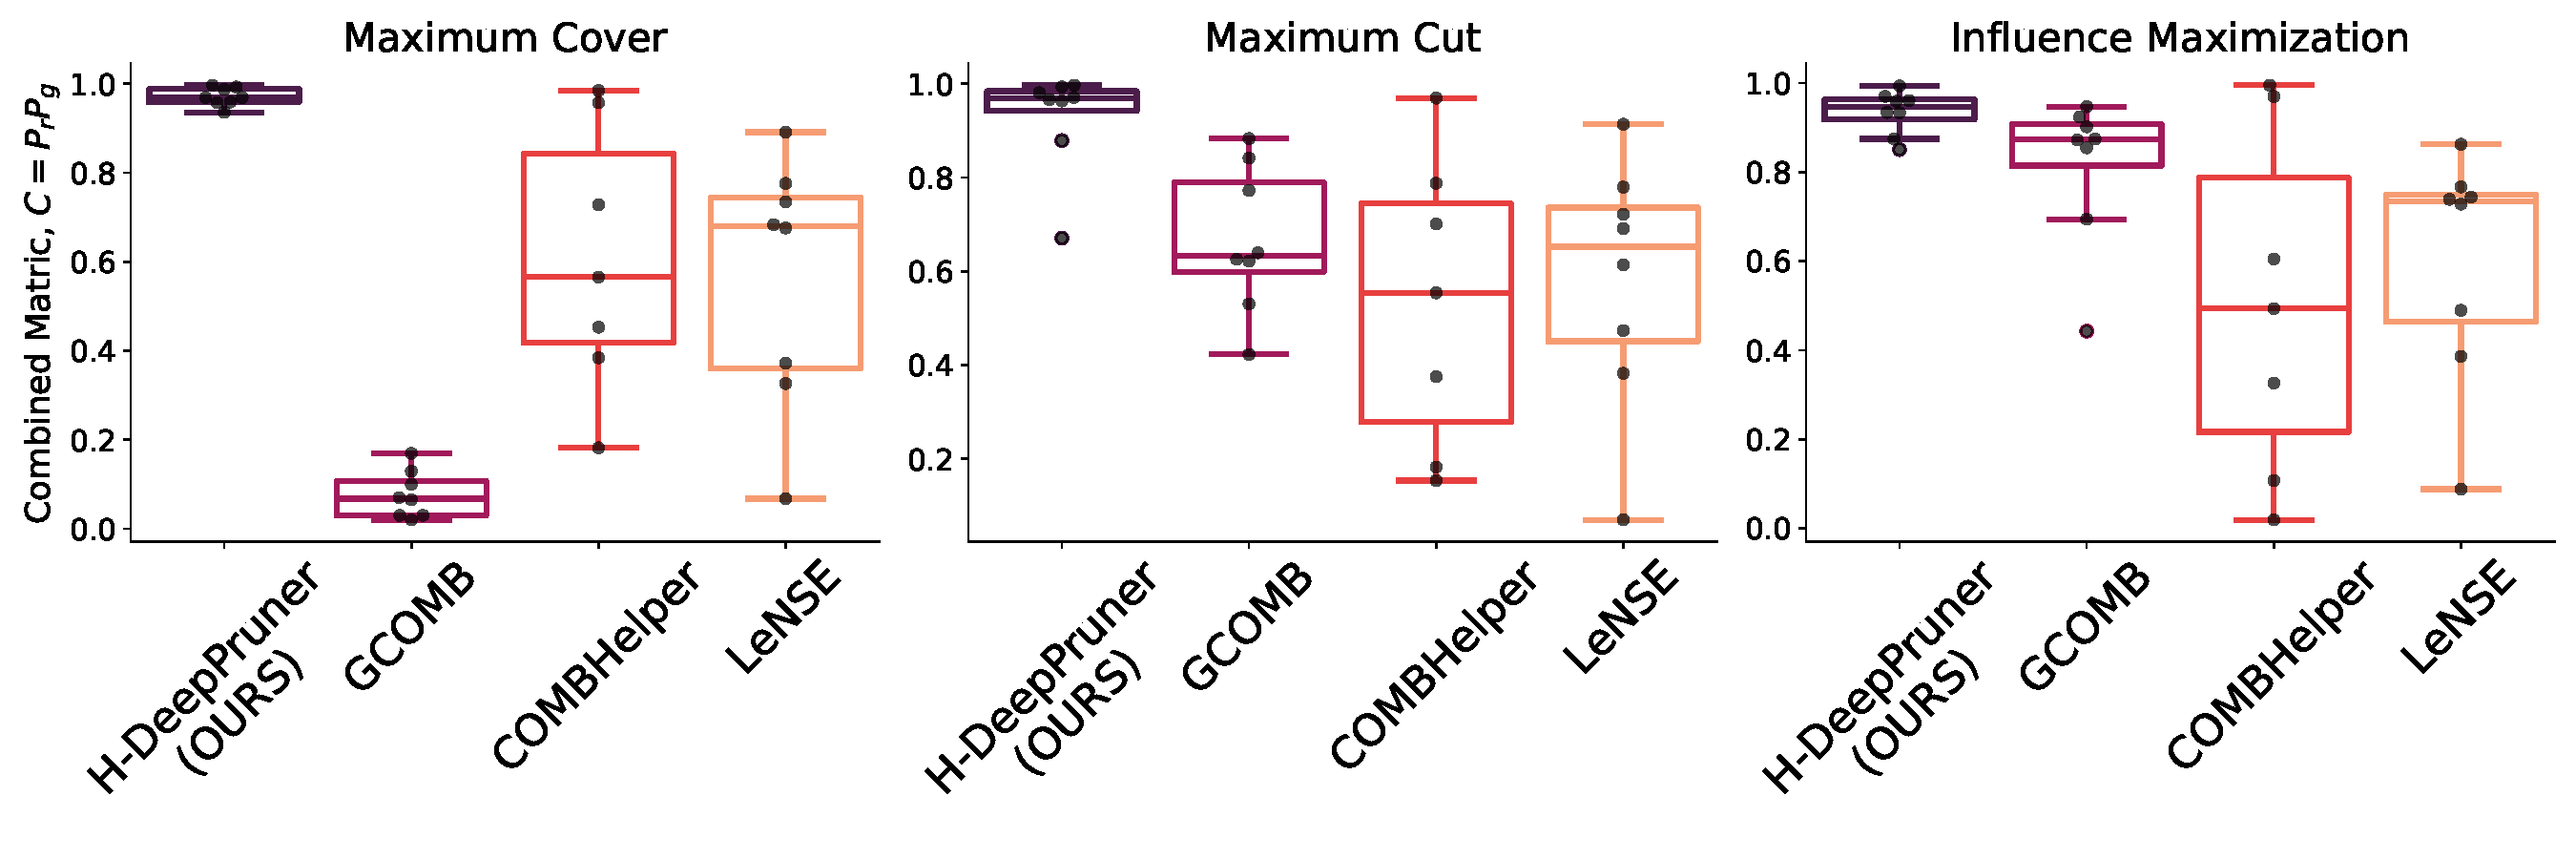
\includegraphics[width=\linewidth]{logos/violin_plots.pdf}
    % \caption{Caption}
    % \label{fig:placeholder}
\end{figure}
    
\end{frame}


\begin{frame}[plain]{Key Takeaway}



\begin{columns}[T,onlytextwidth]
    % Left Column: Image
    \column{0.3\textwidth}
    \begin{figure}
        \centering
        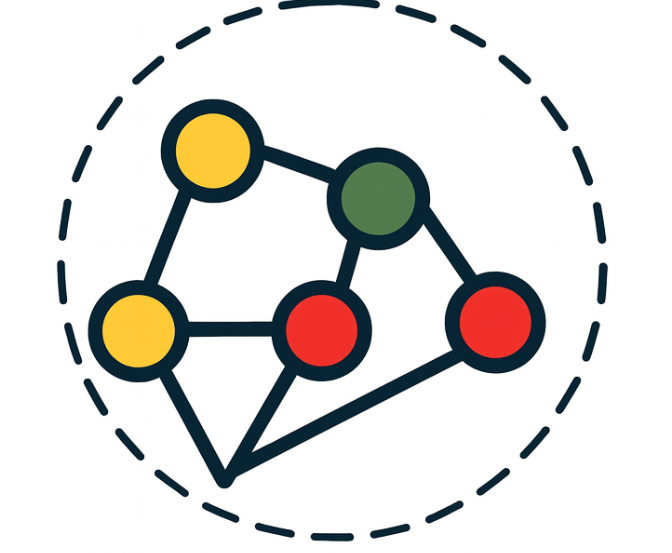
\includegraphics[width=0.9\linewidth]{logos/Pruner.png}
        % \caption{}
    \end{figure}
    Our pruning algorithm is efficient and effective
    % Right Column: Future Work
    \column{0.55\textwidth}
    \textbf{Future Work:}
    \begin{itemize}
        \item Learning algorithms for cases where simple and fast heuristics are ineffective, but pruning improves their performance.
    \end{itemize}
\end{columns}

\end{frame}

\begin{frame}[plain]{References}
  \bibliography{reference.bib}
  \bibliographystyle{plain}
\end{frame}


\end{document}